\documentclass[12pt,a4paper, france]{article}

\newcommand{\workingDate}{\textsc{\selectlanguage{francais}\today}}
\newcommand{\userName}{DM 1}
\newcommand{\institution}{IODAA}
\newcommand\tab[1][1cm]{\hspace*{#1}}
\usepackage{researchdiary_png}


\begin{document}

\begin{center}
{\textbf {\huge DM1 : IA SOLVE}}\\[5mm]
{\large Auguste Gardette} \\[5mm]
{\text{ 20 Octobre 2022}} \\ [5mm]
\end{center}


\section{Recherche d’un chemin optimal par l’algorithme A${^*}$}

Soit le graphe correspondant \`a la figure 1 dans lequel les nombres sur les arcs indiquent le co${\hat{u}}$t
associ\'e \`a cet arc, et les nombres donn\'es pour chaque nœud dans le tableau en haut \`a droite
indiquent la valeur retourn\'e par l\textquoteright heuristique pour ce nœud et le but « G ». \\

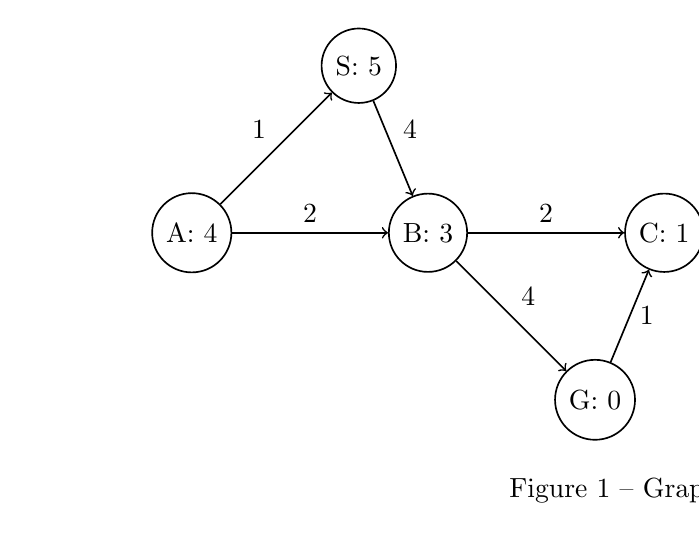
\begin{tikzpicture}[auto, node distance=3cm,semithick, main/.style = {draw, circle}]
\tab \node[main] (1) {A: 4}; 
\node[main] (2) [right of=1] {B: 3}; 
\node[main] (3) [right of=2] {C: 1}; 
\node[main] (4) [above right of=1] {S: 5}; 
\node[main] (5) [below right of=2] {G: 0}; 
\node[below = 10] at (current bounding box.south) {\tab \tab \tab \tab \tab Figure 1 – Graphe.};
\path [->]  (1) edge node {2} (2);
\path [->]  (2) edge node {2} (3);
\path [->]  (1) edge node {1} (4);
\path [->]  (4) edge node {4} (2);
\path [->]  (2) edge node {4} (5);
\path [->]  (5) edge node[right] {1} (3);
\end{tikzpicture} \\ [5mm]

Donnez l\textquoteright ordre d\textquoteright exploration des nœuds d\'evelopp\'es par une recherche en meilleur d\textquoteright abord commençant par le nœud  « S ». Montrez l\textquoteright \'evolution des listes OUVERT et FERM\'E. \\

\section{Optimalit\'e de l\textquoteright algorithme A${^*}$}

Prouvez que l\textquoteright algorithme A${^*}$ retourne un chemin de co${\hat(u)}$t optimal si la fonction heuristique h(n) est admissible. \\

\section{Transformation de A${^*}$ pour trouver un chemin le plus long}

L\textquoteright algorithme A${^*}$  permet de trouver un plus court chemin dans un graphe. On va chercher ici
comment le transformer pour qu\textquoteright il permette de trouver un plus long chemin. \\

1. Que se passe-t-il si on n\textquoteright utilise pas de fonction heuristique ? \\
\tab 2. Quelle doit ${\hat(e)}$tre la propri\'et\'e d\textquoteright une fonction heuristique pour que le chemin retourn\'e soit un plus long chemin ? \\
\tab 3. Donner l\textquoteright algorithme retournant un plus long chemin. \\
\tab 4. Le tester sur le petit graphe de la figure 1 et montrer l\textquoteright ordre d\textquoteright exploration des nœuds. \\

\section{Jeu à trois joueurs}

Comment pourrait-on modifier l\textquoteright algorithme minimax pour qu\textquoteright il soit utilisable dans le cas d\textquoteright un jeu \`a information parfaite \`a trois joueurs ? \\
Par exemple, consid\'erons un jeu \`a trois joueurs nomm\'es 0, 1 et 2 (voir figure 2). On va supposer que la fonction d\textquoteright \'evaluation retourne un triplet de valeurs indiquant l\textquoteright \'evaluation de la position pour les joueurs 0, 1 et 2. Par exemple, le triplet (6, 2, 4) indique que cette position est tr\`es d\'esirable pour le joueur 0, nettement moins pour le joueur 1 et moyennement pour le joueur 2.\\

1. Compl\'eter l’arbre de jeu de la figure 2 en remplissant les triplets jusqu\textquoteright \`a la racine.\\
\tab 2. R\'e-\'ecrire le programme MinMax pour qu\textquoteright il joue correctement sur ce type d\textquoteright arbre. \\

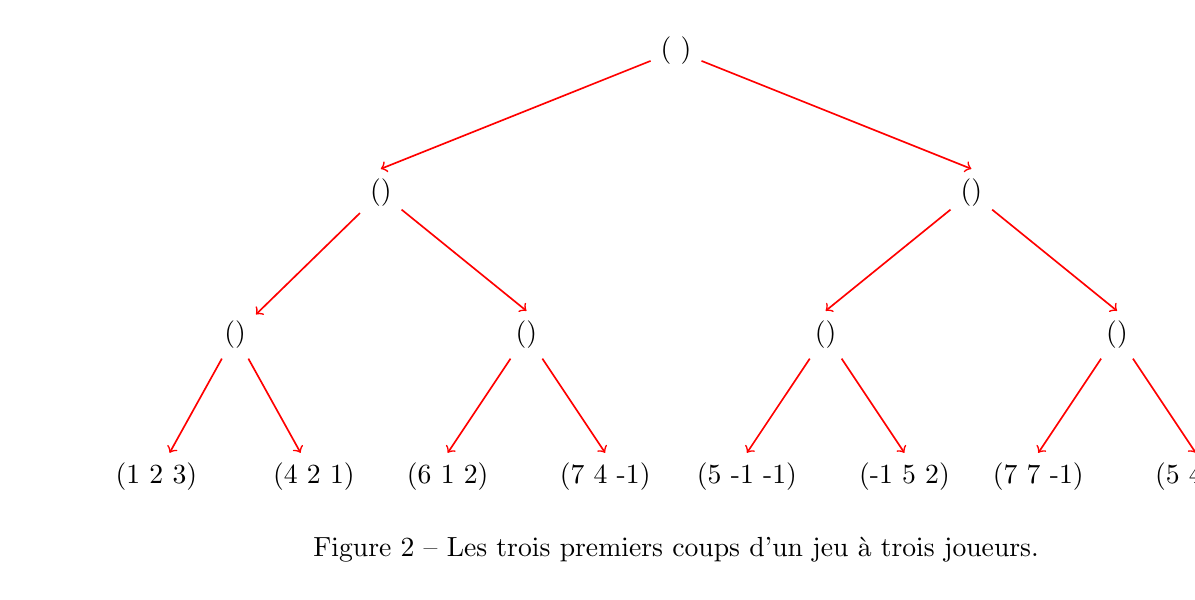
\begin{tikzpicture}[auto, node distance=3.4cm,semithick, level 1/.style={sibling distance=7.5cm},
level 2/.style={sibling distance=3.7cm}, level 3/.style={sibling distance=2cm}, level 4/.style={sibling distance=1.3cm}]
\tab \node (1) {(    )}
    child{[draw=red, ->] node [below] {()}
        child{  node [below] {()}
            child{ node [below] {(1 2 3)} 
            } 
            child{ node [below] {(4 2 1)}
            }
        }
        child{[->] node [below] {()}
            child{ [->] node [below] {(6 1 2)}
            }
            child{[->] node [below] {(7 4 -1)}
            }
        }
    }
    child{[draw=red, ->] node [below] {()}
        child{[->] node [below] {()}
            child{ [->] node [below] {(5 -1 -1)}
            }
            child{[->] node [below] {(-1 5 2)}
            }
        }
        child{[->] node [below] {()}
            child{ [->] node [below] {(7 7 -1)}
            }
            child{[->] node [below] {(5 4 5)}
            }
        }
    };
\node[below = 10] at (current bounding box.south) {Figure 2 – Les trois premiers coups d’un jeu à trois joueurs.};
\end{tikzpicture} \\ [5mm]

\end{document}

